\documentclass{article}
\usepackage[english, russian]{babel}
\usepackage{ucs}
\usepackage[letterpaper,top=2cm,bottom=2cm,left=3cm,right=3cm,marginparwidth=1.75cm]{geometry}
\usepackage{amsmath}
\usepackage{graphicx}
\usepackage[colorlinks=true, allcolors=blue]{hyperref}
\usepackage[utf8x]{inputenc}
\usepackage[T2A]{fontenc}
\usepackage{hyphenat}
\usepackage{float}
\usepackage{wrapfig}
\usepackage{mathtools}

\author{Самойлов Михаил, Ларионов Захар}
\title{Кинетика взаимодействия фенолфталеина с NaOH:\\
определение порядков реакции,\\ изучение влияния ионной силы раствора}
\date{9 февраля 2024}
\begin{document}
\maketitle 
\begin{figure}[b]
    \centering
    \includegraphics[width=0.5\linewidth]{logo.png}
\end{figure}
\newpage

\section{Цель работы}
\begin{enumerate}
    \item Определение порядка реакции по исследуемому красителю и по NaOH, расчёт констант скорости реакции.
    \item Исследование влияния ионной силы раствора на скорость реакции.
\end{enumerate}


\section{Задачи}
\begin{enumerate}
    \item Исследовать порядок реакции по красителю 
    \item Определить $k_1$, $k_2$
    \item Исследовать скорость реакции в зависимости от ионной силы раствора 
\end{enumerate}

\section{Теоретическая справка}
\subsection{Общие сведенья о исследумом красителе}
Метиловый фиолетовый - трифенильный краситель с формулой $C_{25}H_{30}N_3Cl$.

\begin{figure}[H]
    \centering
    \includegraphics[width=0.5\linewidth]{metil2.png}
    \captionof{Рисунок 1: Структурная формула метилового фиолетового}
    \label{fig:enter-label}
\end{figure}

Но в данной работе нам этого не надо. Надо знать только то, что от этого динозавра можно оторавть 2 протона, т.е. формулу соединения можно представить как $H_2P$
В такой форме метиловый фиолетовый присутствует в растворе при $pH \approx 8$. В диапазоне pH > 8 форма нашего красителя представима в виде $P^{-2}$. Такие ионы обладают фиолетовой окраской. При дальнейшем увеличении pH начинается реакция обесцвечивания:
\begin{gather}
    P^{-2} + OH^- \rightleftharpoons POH^3-
\end{gather}
В данной работе изучена кинетика протекания данной реакции при различных концентрациях NaOH и ионной силы раствора.

\subsection{Зависимость скорости реакции от концентрации NaOH}
 Взяв большой изыбток щелочи по отношению к реагирующему красителю, можно считать её концентрацию приблизительно постоянной в ходе реакции и определить порядок по красителю:
\begin{gather}
    \frac{d[A]}{dt} = k_2 [A]^{P_A}[OH^-]^{P_{OH^-}} = k_1[A]^{P_A}
\end{gather}
где [A] - концентрация красителя, $P_i$ - соответствующие порядки реакции, $k_1 = k_2[OH^-]^{P_{OH^-}} \approx const$ во время реакции. Из закона светопоглащения Бугера-Ламберта-Бера имеем:
\begin{gather}
    D = \epsilon_{\lambda}l[A]
\end{gather}
где $\epsilon_{\lambda}$ - коэффициент экстинции при данной длине волны волны, D - оптическая плотность, l - толщина слоя вещества. Предполагая первый порядок реакции по красителю, можно получить решение кинетического уравнения в виде:
\begin{gather}
    [A] = [A]_0exp(-k_1t)
\end{gather}
Из уравнений (2) и (3) после преобразования получим:
\begin{gather}
    lnD = -k_1t + lnD_0
\end{gather}
Соответственно по углу наклона $\frac{dlnD}{dt}$ можно определить значение k1.
\subsection{Зависимость скорости реакции от ионной силы раствора}
Константа скорости реакции должна зависеть от ионной силы раствора. Зависимость должна подчиняться уравнению Брендстеда-Бьеррума:
\begin{gather}
    lg(\frac{k}{k_0}) = 1,02 \cdot Z_AZ_BI^{\frac{1}{2}}
\end{gather}
Анализ полученного выражения показывает, что в случае одноименно заряженных ионов($Z_AZ_B > 0$) константа скорости реакции растёт с ионной силой, тогда как в случае разноимённых ($Z_AZ_B < 0$) - уменьшается. Зависимость скорости реакций с растворах от ионной силы носит название \textit{первичного солевого эффекта}, причем знак и маштаб влияния J на скорость реакции позволяют установить заряжность частиц, участвующих в лимитирующей стадии процесса, по наклону графиков $lg(k/k_0)$ oт $J^{1/2}$


\section{Методика эксперимента}

\subsection{Снятие спектра исследуемого красителя}
В ходе работы был исследован краситель:
метиловый фиолетовый $C_{25}H_{30}N_3Cl$. В данном пункте были приготовлены разбавленные водные растворы красителя, сняты спектры поглощения в интервале 300-700 нм. По полученнным данным можно определить пик поглощения для дальнейших опытов. Для метилового фиолетового максимум оптической плотности наблюдается при длине волны $\lambda_ {mf} = 590$, что согласуется с теоритическими значениями.
\begin{figure}[H]
    \centering
    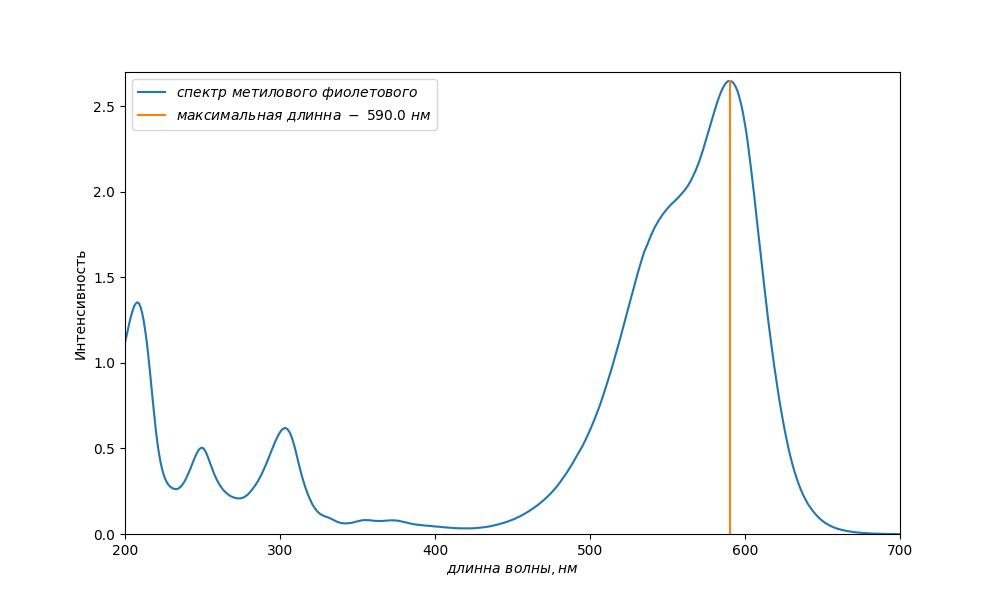
\includegraphics[width=1\linewidth]{kin_wave.jpg}
    \caption{График для определения \lambda_{max}}
\end{figure}

\subsection{Исследование зависимости скорости обесцвечивания от концентрции щёлочи}
В этом пункте были проведены измерения кинетической кривой обесцвечивания D(t) при различных концентрациях NaOH и фиксированной ионной силе I, постоянство которой достигалась добавлением индефирентного электролита.
Полученные с помощью спектрофотометра кинетические кривые линеризуем в полулогарифмичесикх координатах и с помощью numpy найдём значения $k_1$(рисунок 1, 2).После этого построим графики зависимостей определенных через numpy $k_1$ от $[OH^-]$ в логарифмических координатах, чтобы определить порядок реакции по красителю (рис.3,4).

\subsection{Исследование зависимости скорости обесцвечивания от ионной силы раствора}
Построим график зависимости D(t) в линеризирующих координатах и по этим данным найдём k, и исследуем её отношение к $Z_AZ_B$


\section{Практическая часть}
\subsection{Определение порядков реакции}

Снимем спектры сигналов при разной концентрации $NaOH$. Для этих графиков линнеариацией будут координаты натурального логарифма. 

\begin{figure}[H]
    \centering
    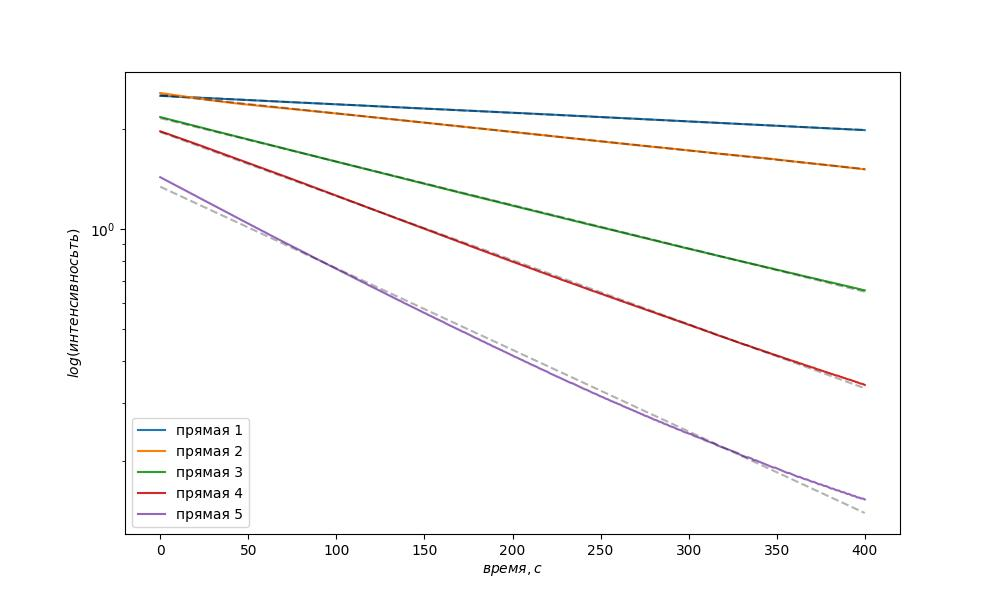
\includegraphics[width=1\linewidth]{expo.jpg}
    \caption{График в линеаризующих координатах}
\end{figure}
Данный график построен опираясь на рассуждения, приведенные выше.


\begin{table}[H]
    \centering
    \begin{tabular}{|c|c|c|c|c|c|} \hline
         & расствор 1 & расствор 2 & расствор 3 & расствор 4 & расствор 5\\ \hline
         V_{NaOH}, \text{мл} & 0.1 & 0.2 & 0.4 & 0.6 & 0.8\\ \hline
         V_{NaCl}, \text{мл} & 0.9 & 0.8 & 0.6 & 0.4 & 0.2\\ \hline
         k прямой& -0.00059 & -0.0013 & -0.0030 & -0.0045 & -0.0057 \\ \hline
         MSE & 0.086 & 0.148 & 0.108 & 0.125 & 0.343\\ \hline
    \end{tabular}
    \caption{соответствие характеристик и расстворов по номерам}
\end{table}

\begin{figure}[H]
    \centering
    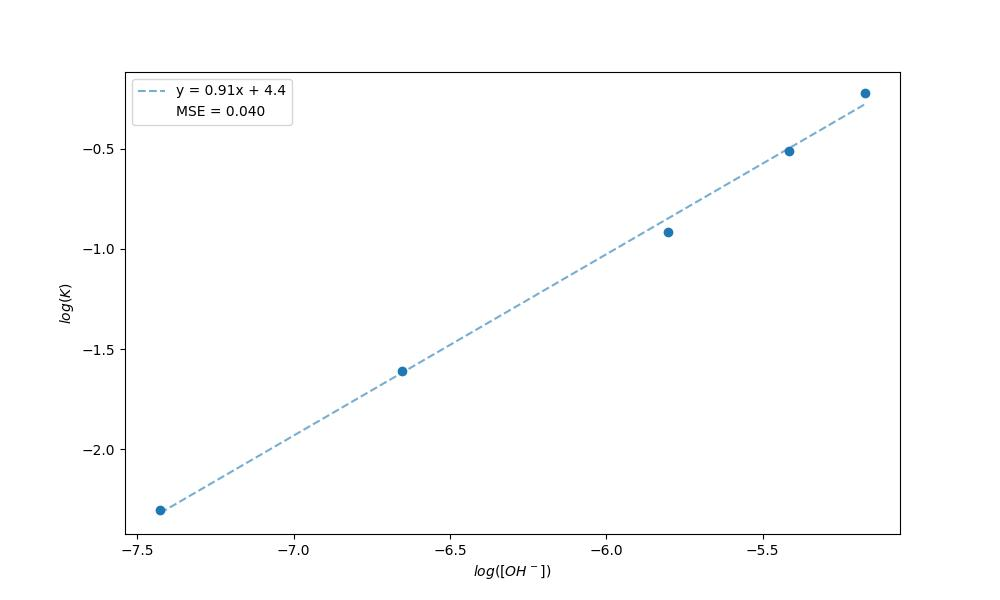
\includegraphics[width=1\linewidth]{stepeni.jpg}
    \caption{График зависимости log(K)(log([OH^-]))}
\end{figure}

Сделаем вывод о коэфецинете реакции с метиловым фиолетовым. \\Степень реакции по $[OH^-] \text{ равняется } 0.91 \approx 1$ 

\begin{center}
    $k_2$ = exp(-4.397) = 0.0123 $M^{-1}c^{-1}$
\end{center}


\subsection{Зависимость от ионной силы}

Теперь измерим кинетические кривые при фиксированной концентрации NaOH, но при разной ионной силе.
\begin{figure}[H]
    \centering
    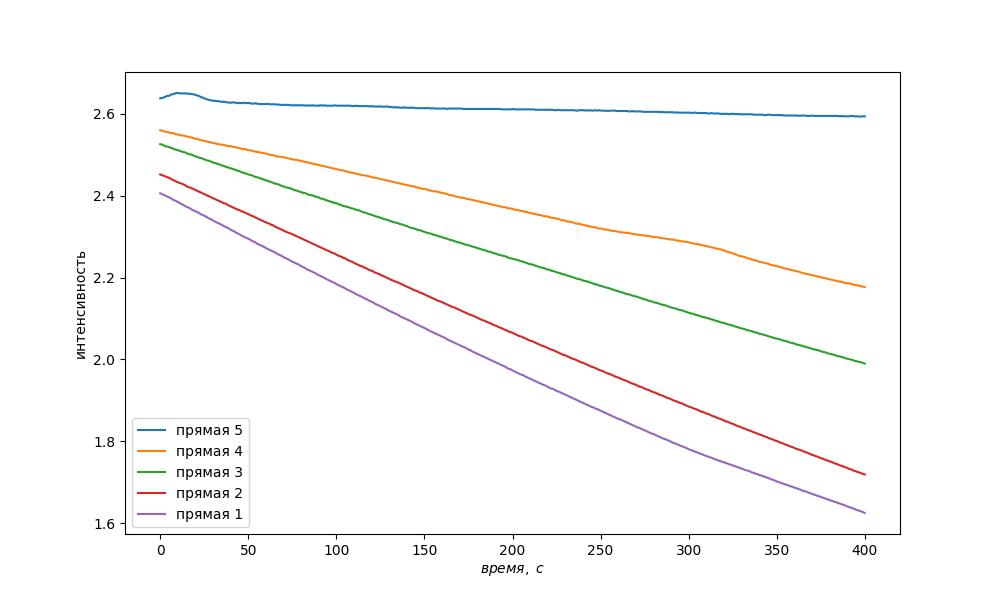
\includegraphics[width=1\linewidth]{pic2_1.jpg}
    \caption{Сырые данные второго эксперимента}
\end{figure}

\begin{figure}[H]
    \centering
    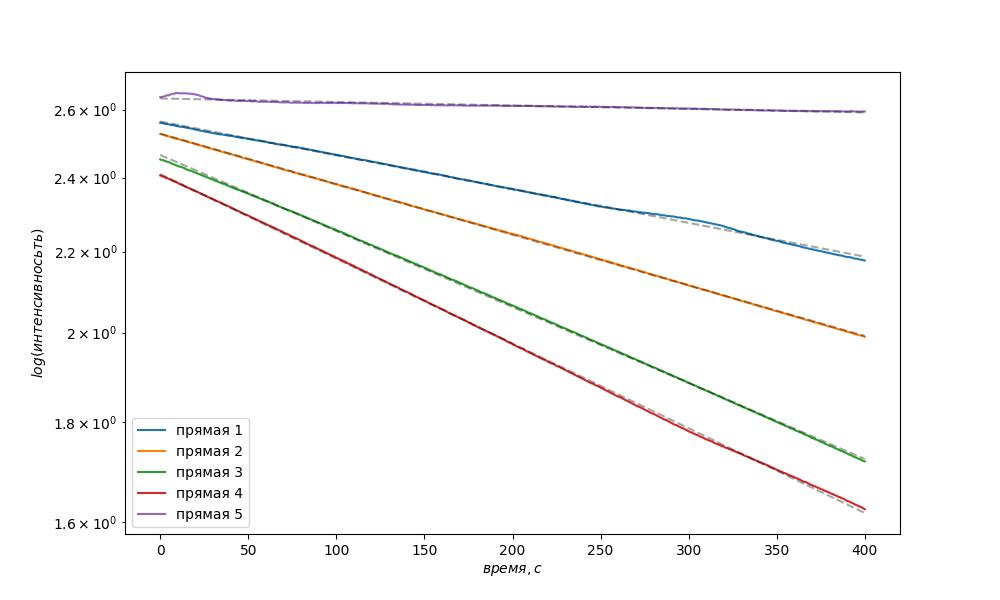
\includegraphics[width=1\linewidth]{pic2_2.jpg}
    \caption{График в линеаризующих координатах}
\end{figure}


\begin{table}[H]
    \centering
    \begin{tabular}{|c|c|c|c|c|c|} \hline
         & раствор 1 & раствор 2 & раствор 3 & раствор 4 & раствор 5\\ \hline
         Ионная сила & 0.01 & 0.0368 & 0.3 & 0.8 & 0.04\\ \hline
         k прямой * $10^{-4}$& -3.97 & -5.95 & -8.94 & -9.96 & -0.41 \\ \hline
         MSE & 0.063 & 0.086 & 0.110 & 0.114 & 0.0088\\ \hline
    \end{tabular}
    \caption{Информация о растворах}
\end{table}

Несмотря на то, что раствор 5 должен был расположиться между 2 и 3 мы добавили его именно под этим номером. Дело в том, что по графикам это значение похоже на типичный выпад. Точно восстановить причину этого не предоставляется возможным, но по коэфиценту наклона можно предположить, что была нарушена процедура подготовки расствора. Либо были перепутаны какие-либо реактивы, либо просто не добавлены, либо добавлены в намного меньшем объеме, ибо реакция почти не идет, несмотря на то, что по значению ионной силы это не минимальное значение.

Теперь построим график зависимости константы от корня ионной силы. Более подробно написано в теоретической справке.

\begin{figure}[H]
    \centering
    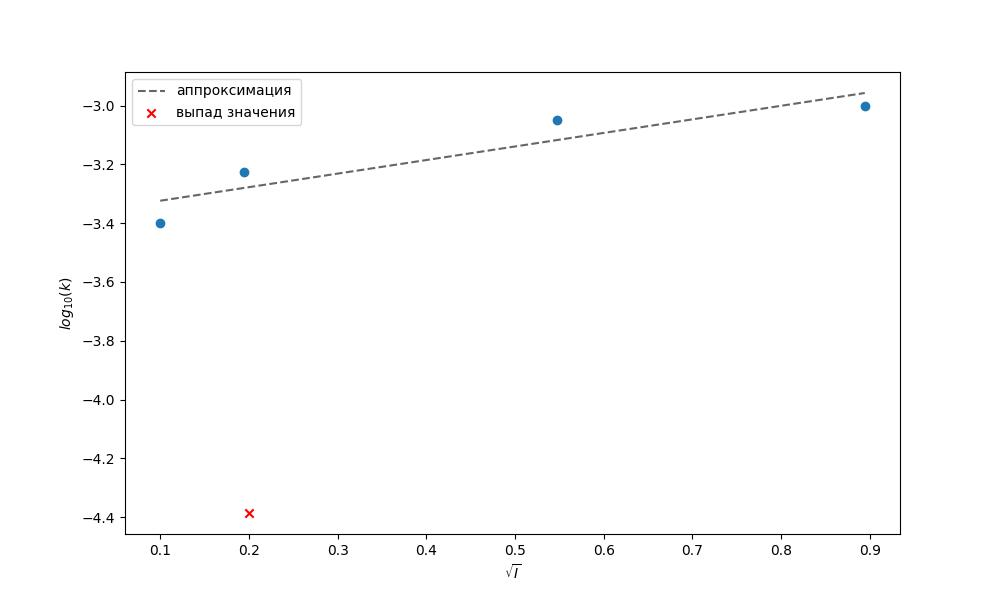
\includegraphics[width=1\linewidth]{pic2_3.jpg}
    \caption{Зависимость констант скорости от ионной силы}
\end{figure}

Регрессионная прямая имеет формулу:
\begin{center}
    $y = 0.462x - 3.37$
\end{center}

Значит для метилового фиалетового мы получили значение
\begin{center}
    $Z_aZ_b = 0.462$
\end{center}

\section{Вывод}
В ходе данной работы были изученые кинетически порядки реакций компонентов. Частный порядок реакции по $[OH^-]$ составил 1, как и по красителю.В том числе была посчитана константа скорости данной реакции при фиксированной ионной силе.Также была исследована зависимость константы скорости реакции от ионной силы. Мы получили, что с ростом ионной силы константа скорости реакции растёт, как $10^k(I)$, что подтверждает уравнение Бренстеда-Бьеррума.




\end{document}